% Submission report, drafted from the contest template.
% Compile from model-report/:  latexmk -pdf report.tex
% Four pages through Limitations. Outside data and the appendix are extra.
\documentclass[11pt]{article}
\usepackage[margin=1.7cm]{geometry}
\usepackage{amsmath,booktabs,array,graphicx,caption,enumitem,placeins,titlesec}
\usepackage[hidelinks]{hyperref}
\usepackage{tikz}
\usetikzlibrary{arrows.meta}

\graphicspath{{figures/}{../figures/}}
\setlist[itemize]{topsep=2pt,itemsep=1pt,leftmargin=1.15em}
\captionsetup{font=small,labelfont=bf,skip=4pt}
\setlength{\parskip}{2pt}
\titlespacing*{\section}{0pt}{8pt}{3pt}
\titlespacing*{\subsection}{0pt}{6pt}{2pt}
\setlength{\parindent}{0pt}
\definecolor{navy}{HTML}{1F4E79}
\pagestyle{plain}

\title{SSU Data Dash 2026: \textit{Team name}}
\author{Amy Dang Phuong, Maira Masroor, Shannon Tanoto, Yiwei Jiang}
\date{}

\begin{document}
\maketitle
\vspace{-10pt}

\noindent\begin{tabular}{@{}l l@{}}
\textbf{Video (YouTube, unlisted is fine):} & \url{https://youtu.be/YOUR-VIDEO} \\
\textbf{Code and submission files (GitHub):} & \url{https://github.com/YOUR-TEAM/YOUR-REPO} \\
\end{tabular}

\section*{Summary}

We answer two questions with two models, and we do not mix the scores. A desk that can see the listing gets a close: walk-forward median absolute percentage error \(4.28\%\), against \(7.26\%\) for taking the ask as the forecast, with the typical prediction still \(0.9\%\) high. A desk marking a home before anyone has published an ask gets a value: walk-forward MdAPE \(7.45\%\), against \(15.33\%\) for a 12-month community dollars-per-square-foot anchor. Off-market counts double. The list price correlates \(0.986\) with the sold price, so the tighter number is the ask.

The accuracy is in the columns and in one calibration, not in a retuned tree. Both models are one LightGBM on a log target, with the same settings, fit only on sales that have already closed. The list-aware model predicts the gap around the ask. A regression and a SARIMAX turn the market's drift into a column, and the tree decides the pass-through. The off-market model builds the level from a local tape, same-building sales brought forward to the listing month, and a remarks score fit out of time, then applies one shift from the prior three months. The failures point opposite ways. The list-aware model is rich on cheap homes. The off-market model is cheap on expensive homes, and cheap again when the tape goes stale.

\section{Data and features}

The book is \(150{,}000\) synthetic Toronto sales, January 2021 through May 2026. Names and coordinates do not match real maps, so we join nothing. Outside data: none. Both models see the same \(10{,}069\) validation sales, December 2025 through May 2026, and both are refused any sale that had not closed yet. An inner slice, July through November 2025, is where we froze the windows, the phrases, the building rule, and the shift weight. Those months then go back into the estimation sample. The walk-forward is the number we quote, because it never scores a month the tree has seen.

Every model sees log floor area (the midpoint when the listing wrote a range), a lot-missing flag, log frontage, depth, beds, baths, parking, garage, latitude, longitude, the listing month as a sine and cosine, and type, style, municipality, and community. Lot size is missing on every condo and present on every house, so the flag is a house-versus-apartment cut. A cell with fewer than 30 past sales falls back, community to type to city. An unseen category stays missing. The equations for the columns below are in Appendix~\ref{app:la} and Appendix~\ref{app:om}.

\subsection{List-aware}

\begin{center}
\small
\begin{tabular}{p{4.4cm}p{11.2cm}}
\toprule
Column & What it is \\
\midrule
Log ask, lot area, area-was-a-range & The ask, and a flag when size was written as a range. \\
Peer ask & List \$/sqft divided by median sold \$/sqft, same community and type, closed before the listing month. \\
Three-month discount & Median sold/list in that cell over the three prior sale months. Missing on \(46\%\) of a frozen fit. \\
City lag & Median log gap in the previous calendar month. \\
Month factor & SARIMAX forecast of the monthly mean residual from a log-linear fit on the ask. \\
\bottomrule
\end{tabular}
\end{center}

Split gain on the fitted tree: peer ask \(22\%\), community \(19\%\), log ask \(10\%\), city lag \(9\%\), three-month discount \(8\%\), month factor \(6\%\). The lot-missing flag is \(0.07\%\), because the ask has already named the product. Remarks, tried as a text decomposition, moved developmental MdAPE from \(4.83\%\) to \(4.85\%\), so this track has no text (Appendix~\ref{app:drop-la}).

\subsection{Off-market}

\begin{center}
\small
\begin{tabular}{p{4.4cm}p{11.2cm}}
\toprule
Column & What it is \\
\midrule
12-month community \$/sqft & Median sold \$/sqft, same community and type, prior 12 months. The level the ask would have carried. \\
City \$/sqft, 3 and 12 months & The same median, citywide, at two windows. \\
Building price and count & Same pin and type, closed before listing, reindexed to the listing month. Present for \(60\%\) of validation homes. \\
Thirteen phrase flags & Written patterns in the remarks. Not a fitted model. \\
Remarks score & A ridge of log price on the description. Each training row is scored by earlier sales only. \\
\bottomrule
\end{tabular}
\end{center}

Split gain: lot missing \(33\%\), building price \(18\%\), log size \(13\%\), community \(12\%\), log frontage \(8\%\). The remarks score is \(0.7\%\). The comps are doing the work. Municipality is about zero once community is in the tree.

\section{Models}

Same tree, two targets. LightGBM, squared error, 127 leaves, learning rate \(0.03\), 700 trees, at least 20 rows in a leaf, row and column subsamples \(0.8\), L2 penalty \(1\), seed \(0\). We did not reopen that grid after the list-aware target became the log gap. Retuning an earlier specification on July--November and then refitting produced a December--May MdAPE of \(4.57\%\), worse than the untuned \(4.53\%\).

\subsection{List-aware}

The target is \(\log(\mathrm{sold}/\mathrm{list})\). The price is the ask times \(\exp(\mathrm{gap})\). The month factor is a column, \(6.3\%\) of gain, and the tree is the last step. A level shift after the tree won one frozen window and then sat \(1.75\%\) low on the walk. We did not adopt it (Appendix~\ref{app:drop-la}).

\subsection{Off-market}

The target is \(\log(\mathrm{sold})\). The price is then multiplied by \(\exp(-\delta)\) at full weight. \(\delta\) is the median log miss on the three months before the origin, from a tree that did not see those months, and the walk re-estimates it every month. On the July--November screen, no shift was MdAPE \(8.31\) and \(+4.71\%\) high. Full weight was \(7.97\) and \(+3.77\%\). On the one-origin fit, \(\delta=+1.58\%\). A model that starts from the community anchor reached walk-forward MdAPE \(7.50\). The direct model is ahead in five months, and February is the loss (Appendix~\ref{app:months}). We kept the direct model because it won the screen and then held the walk.

\begin{figure}[ht]
\centering
\begin{minipage}[t]{0.48\linewidth}
\centering
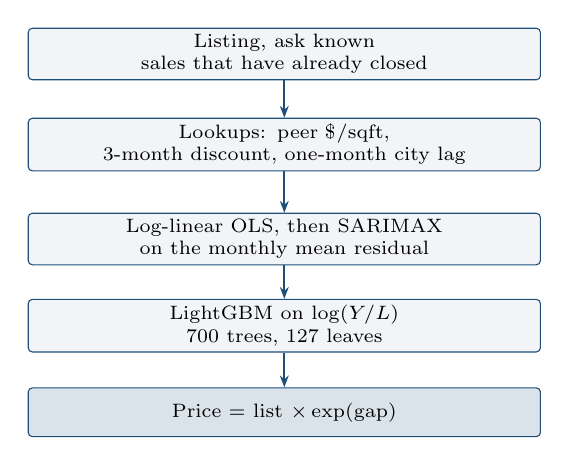
\begin{tikzpicture}[
  font=\scriptsize,
  box/.style={draw=navy, rounded corners=1.5pt, align=center, inner sep=2.2pt,
              fill=navy!6, text width=6.35cm, minimum height=6.2mm},
  arr/.style={-{Stealth[length=1.5mm]}, semithick, draw=navy}
]
\node[box] (a) at (0,0) {Listing, ask known\\ sales that have already closed};
\node[box] (b) at (0,-1.15) {Lookups: peer \$/sqft,\\ 3-month discount, one-month city lag};
\node[box] (c) at (0,-2.35) {Log-linear OLS, then SARIMAX\\ on the monthly mean residual};
\node[box] (d) at (0,-3.45) {LightGBM on \(\log(Y/L)\)\\ 700 trees, 127 leaves};
\node[box, fill=navy!16] (e) at (0,-4.55) {Price \(=\) list \(\times\exp(\mathrm{gap})\)};
\draw[arr] (a) -- (b); \draw[arr] (b) -- (c);
\draw[arr] (c) -- (d); \draw[arr] (d) -- (e);
\end{tikzpicture}\\[2pt]
{\small\textbf{List-aware.} The SARIMAX is one column. The tree is the last step.}
\end{minipage}\hfill
\begin{minipage}[t]{0.48\linewidth}
\centering
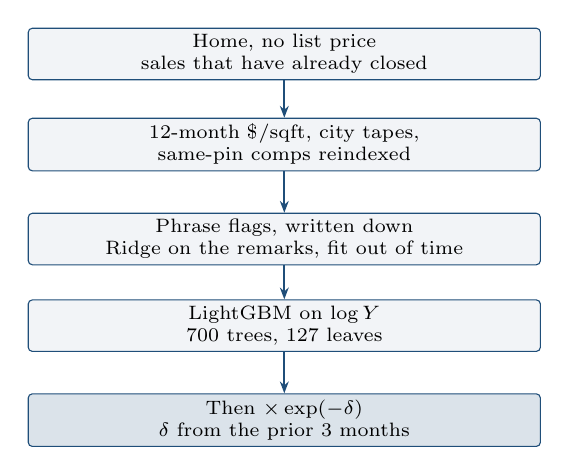
\begin{tikzpicture}[
  font=\scriptsize,
  box/.style={draw=navy, rounded corners=1.5pt, align=center, inner sep=2.2pt,
              fill=navy!6, text width=6.35cm, minimum height=6.2mm},
  arr/.style={-{Stealth[length=1.5mm]}, semithick, draw=navy}
]
\node[box] (a) at (0,0) {Home, no list price\\ sales that have already closed};
\node[box] (b) at (0,-1.15) {12-month \$/sqft, city tapes,\\ same-pin comps reindexed};
\node[box] (c) at (0,-2.35) {Phrase flags, written down\\ Ridge on the remarks, fit out of time};
\node[box] (d) at (0,-3.45) {LightGBM on \(\log Y\)\\ 700 trees, 127 leaves};
\node[box, fill=navy!16] (e) at (0,-4.65) {Then \(\times\exp(-\delta)\)\\ \(\delta\) from the prior 3 months};
\draw[arr] (a) -- (b); \draw[arr] (b) -- (c);
\draw[arr] (c) -- (d); \draw[arr] (d) -- (e);
\end{tikzpicture}\\[2pt]
{\small\textbf{Off-market.} Flags are patterns. The ridge is a model. \(\delta\) is the only second stage.}
\end{minipage}
\caption{Scoring path for each subsection above. The list-aware chain ends at the tree. The off-market chain has one shift after it.}
\label{fig:each}
\end{figure}

% \subsection{Both paths}

% Figure~\ref{fig:both} starts from the shared attributes. The lookups, the SARIMAX, and the ridge are columns into one tree on each track.

% \begin{figure}[ht]
% \centering
% \begin{tikzpicture}[
%   font=\scriptsize,
%   box/.style={draw=navy, rounded corners=1.5pt, align=center, inner sep=2.2pt,
%               fill=navy!6, text width=6.3cm, minimum height=6.4mm},
%   arr/.style={-{Stealth[length=1.5mm]}, semithick, draw=navy}
% ]
% \node[box, text width=9.2cm] (raw) at (0,0) {Home, plus sales that have already closed};
% \node[box, text width=9.2cm, fill=navy!4] (shared) at (0,-1.2)
%   {Shared attributes: log size, lot, rooms, coordinates, month, type, style, place};
% \node[box] (la) at (-3.9,-2.75) {List-aware lookups\\ peer ask, discount, city lag};
% \node[box] (sar) at (-3.9,-4.0) {OLS, then SARIMAX\\ month factor is one column};
% \node[box, fill=navy!16] (out) at (-3.9,-5.15) {LightGBM on \(\log(Y/L)\)\\ price \(=\) list \(\times\exp(\mathrm{gap})\)};
% \node[box] (om) at (3.9,-2.75) {Off-market lookups\\ 12-month tape, pin comps};
% \node[box] (txt) at (3.9,-4.05) {Written flags, and a ridge\\ remarks score is one column};
% \node[box, fill=navy!16] (out2) at (3.9,-5.25) {LightGBM on \(\log Y\)\\ then \(\times\exp(-\delta)\)};
% \draw[arr] (raw) -- (shared);
% \draw[arr] (shared.south) -- (la.north);
% \draw[arr] (shared.south) -- (om.north);
% \draw[arr] (la) -- (sar); \draw[arr] (sar) -- (out);
% \draw[arr] (om) -- (txt); \draw[arr] (txt) -- (out2);
% \end{tikzpicture}
% \caption{The two paths from one front door. The right path never reads the list price. A building comp has to have closed before the home was listed.}
% \label{fig:both}
% \end{figure}

\FloatBarrier
\section{Validation}

The walk is one procedure for both tracks. For each month from December 2025 through May 2026, every table, the SARIMAX, the ridge, the categories, and the tree are rebuilt on sales that closed before that month. The off-market refit also rebuilds \(\delta\) on the three months before the scored month. The month is then scored. Its sold prices are in none of those objects, and on the off-market track the list price is hidden. A building comp still has to predate the home's listing. The July--November choices stay fixed. Pooled MdAPE weights homes equally, so May (\(2{,}291\) sales) outweighs January (\(1{,}058\)). A random split leaks later closes into the peer medians and the building comps. \texttt{run.py validate} is this procedure. The month path is Appendix~\ref{app:months}.

\section{Results}

\begin{center}
\input{../reports/results_table.tex}\\[2pt]
\captionof{table}{Walk-forward, December 2025--May 2026, \(10{,}069\) homes. Brackets: bootstrap 95\% interval, a lower bound because one month moves together.}
\end{center}

Handout bars we did not refit: \(17.7\%\), \(20.8\%\) for ten nearest sales, and \(7.3\%\) for the list price (our refit \(7.26\%\)). The hidden test runs through September 2026 and should land near this table. We did not choose either model on these six months.

\subsection{List-aware}

The model beats the ask in every month. MdAPE stays inside \(3.97\) to \(4.55\). Community is worth \(0.08\) points over the same model without it (\(4.36\%\)), and it is ahead in every month. The month-by-month comparison with the ask is Figure~\ref{fig:la-walk} in the appendix.

\subsection{Off-market}

The model cuts the 12-month community anchor from \(15.33\%\) to \(7.45\%\). The pooled signed error is \(-0.37\%\). That pool is the average of six months that do not share a sign. The comparison with the anchor, month by month, is Figure~\ref{fig:om-walk} in the appendix.

\section{Where the model fails}

\begin{figure}[ht]
\centering
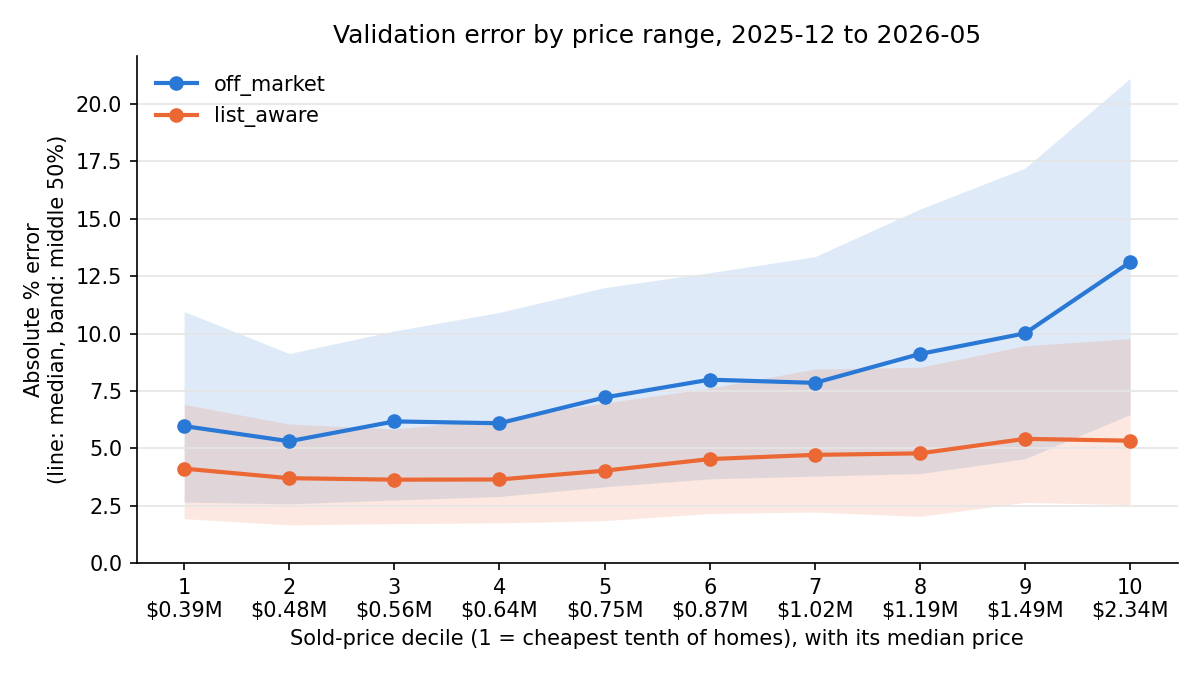
\includegraphics[width=0.48\linewidth]{error_by_price_range.png}
\caption{Walk-forward absolute percentage error by sold-price decile. The line is the median. The band is the middle half of homes.}
\end{figure}

The cheap end is already a bit high on both tracks, so one citywide percent cannot fix either tail.

\subsection{List-aware}

On a one-origin fit the model is \(3.7\%\) high on homes under about \(\$440{,}000\), and close to unbiased in the top decile (MdAPE \(5.6\%\)). Signed error stays positive every month, from \(+0.20\%\) to \(+1.33\%\). Detached and semi-detached cost about two extra points of MdAPE. Across municipalities the error stays inside \(4.2\%\) to \(4.6\%\).

\subsection{Off-market}

The top decile, from about \(\$1.8\) million, has MdAPE \(13.6\%\) and is about \(11\%\) low. Signed error changes sign and reaches \(-4.44\%\) in February (Appendix~\ref{app:months}). Detached and semi-detached cost about three to four extra points of MdAPE, and municipalities stay inside \(6.3\%\) to \(7.7\%\). Scoring May 2026 with the tape cut off at the end of January moves MdAPE from \(7.39\%\) to \(8.38\%\) and the signed error from \(+0.98\%\) to \(-5.29\%\).

\section{Limitations}

Both outputs are a point price. The book is synthetic, the claim stops in May 2026, and the test files run to September.

\subsection{List-aware}

On the one-origin window the 95th percentile of absolute error is about \(14\%\), against \(19\%\) for the ask. We would not add a haircut. The walk-forward already rejected one (Appendix~\ref{app:drop-la}).

\subsection{Off-market}

The 95th percentile is about \(26\%\), against \(57\%\) for the community anchor. A mark above \(\$1.5\) million, or on a tape older than about 90 days, should carry that limit next to the number.


\section*{Reproducing our results}

From a fresh copy of the repository:

\texttt{pip install -r requirements.txt}\\
\texttt{python run.py validate}\\
\texttt{python run.py report}\\
\texttt{python run.py predict}\\
\texttt{python run.py check}

\texttt{validate} writes the walk-forward file. \texttt{report} writes the table and the figure above. \texttt{predict} refits on every closed sale through May 2026, so the off-market shift is then measured on March--May 2026, and writes the two submission files. \texttt{check} confirms one positive finite price per test id.

\newpage
\begin{center}
{\Large\bfseries Appendix}
\end{center}

\noindent The numbered report ends at Limitations. This appendix is separate from those four pages. It holds the formulas (Appendix~\ref{app:la}, Appendix~\ref{app:om}), the month path and the baseline charts (Appendix~\ref{app:months}), and the specifications we measured and did not keep (Appendix~\ref{app:drop-la}, Appendix~\ref{app:drop-om}).

\appendix
\makeatletter
\renewcommand{\@seccntformat}[1]{%
  \ifnum\pdfstrcmp{#1}{section}=0 Appendix \fi
  \csname the#1\endcsname\quad}
\makeatother
\section{List-aware formulas}
\label{app:la}

Peer ask, for a home listed in month \(\tau\), with floor area \(S\) and ask \(L\):
\[
\mathrm{peer\ ask} = \frac{L/S}{m_{c,t}(\tau)},
\]
where \(m_{c,t}(\tau)\) is the median sold dollars per square foot in the same community and type among sales that closed before \(\tau\). Fewer than 30 sales uses the type. The community cell covers \(97\%\) of the developmental validation rows. This is \(22\%\) of list-aware gain.

The month factor starts from a log-linear fit of log sold price on log ask and the attributes. On the estimation sample the ask elasticity is \(0.894\) and \(R^2\) is \(0.966\). We take the monthly mean residual. An augmented Dickey--Fuller test with a trend gives \(p=0.0002\), so we do not difference. The fitted model on the 59 estimation months is a constant, a one-month autoregression, and a 12-month autoregression: intercept \(-0.0046\), AR(1) \(0.872\), seasonal AR(12) \(0.370\). In-sample \(R^2\) on the monthly series is \(0.885\). Putting that forecast back onto the log-linear prediction, as a hard adjustment, cuts developmental MdAPE from \(7.13\%\) to \(4.78\%\) and the median signed error from \(+5.95\%\) to \(+0.25\%\). The tree receives the same number as a column and uses it at a \(6.3\%\) gain share. The median value on the developmental validation rows is \(-0.0539\).

\section{Off-market formulas}
\label{app:om}

The community tape, window \(W=12\), is the median sold dollars per square foot in the same community and type over the prior \(W\) months, then type, then city. We froze 12 months on July--November: MdAPE \(15.33\), against \(16.19\) for 6 months, \(15.70\) for 24, and \(16.42\) with signed error \(+11.97\%\) for the full history. The community cell itself is used for \(76\%\) of developmental validation rows.

A building comp shares the pin, latitude and longitude rounded to six decimals plus property type, closed strictly before the listing date, and is a different listing. Each historical dollars-per-square-foot is stored relative to a type index that uses only earlier months, a three-month median of monthly median log dollars per square foot. At the listing month the comps are brought back to that month's index, and the building price is size times their median. The gate is one prior sale. Requiring three was worse on July--November.

The remarks ridge is log sold price on a bag of unigrams and bigrams, penalty \(0.3\), at most \(3{,}000\) terms, minimum document frequency 40. Numbers and community names are stripped before the vectorizer runs, so the score cannot memorise a printed price or a neighbourhood. Inside the estimation sample each row is scored from sales that closed earlier. July--November preferred the score by \(0.05\) MdAPE, \(7.97\) against \(8.02\).

\section{Walk-forward by month}
\label{app:months}

The two tracks are scored on the same homes, so the months stay in one table. A positive signed error means the prediction is high.

\begin{center}
\small
\begin{tabular}{l r rr rr}
\toprule
 & & \multicolumn{2}{c}{List-aware} & \multicolumn{2}{c}{Off-market} \\
\cmidrule(lr){3-4} \cmidrule(lr){5-6}
Month & Homes & MdAPE & Signed & MdAPE & Signed \\
\midrule
2025-12 & 1{,}238 & 3.97 & \(+1.31\) & 7.42 & \(+0.63\) \\
2026-01 & 1{,}058 & 4.16 & \(+1.33\) & 7.27 & \(-2.50\) \\
2026-02 & 1{,}442 & 4.38 & \(+0.20\) & 8.17 & \(-4.44\) \\
2026-03 & 1{,}816 & 4.14 & \(+0.46\) & 7.10 & \(-1.15\) \\
2026-04 & 2{,}224 & 4.37 & \(+1.31\) & 7.44 & \(+1.65\) \\
2026-05 & 2{,}291 & 4.55 & \(+0.92\) & 7.39 & \(+0.98\) \\
\midrule
Pooled & 10{,}069 & 4.28 & \(+0.90\) & 7.45 & \(-0.37\) \\
\bottomrule
\end{tabular}
\end{center}

\subsection{List-aware}

\begin{center}
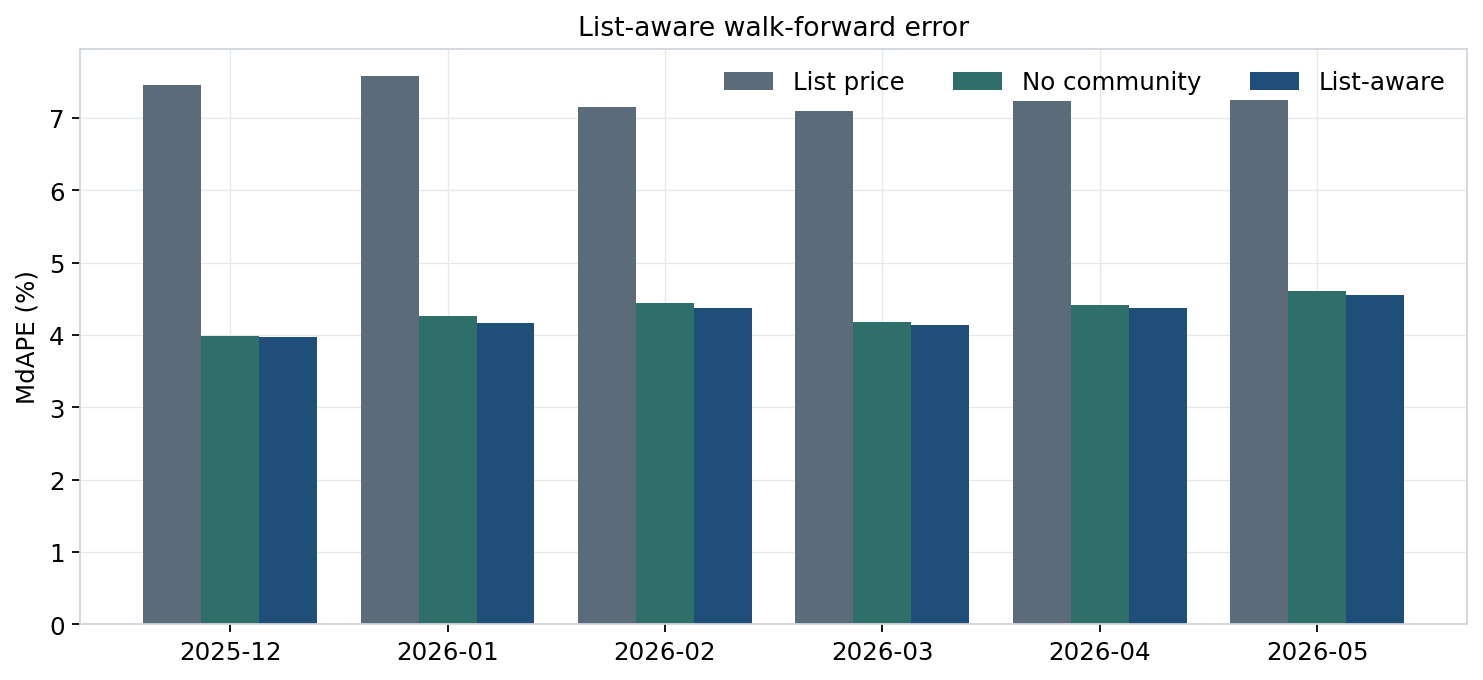
\includegraphics[width=0.92\linewidth]{report_la_mdape.png}
\captionof{figure}{Walk-forward MdAPE by sale month. The list price is the baseline. The middle bar is the same model without community as a category.}
\label{fig:la-walk}
\end{center}

\subsection{Off-market}

\begin{center}
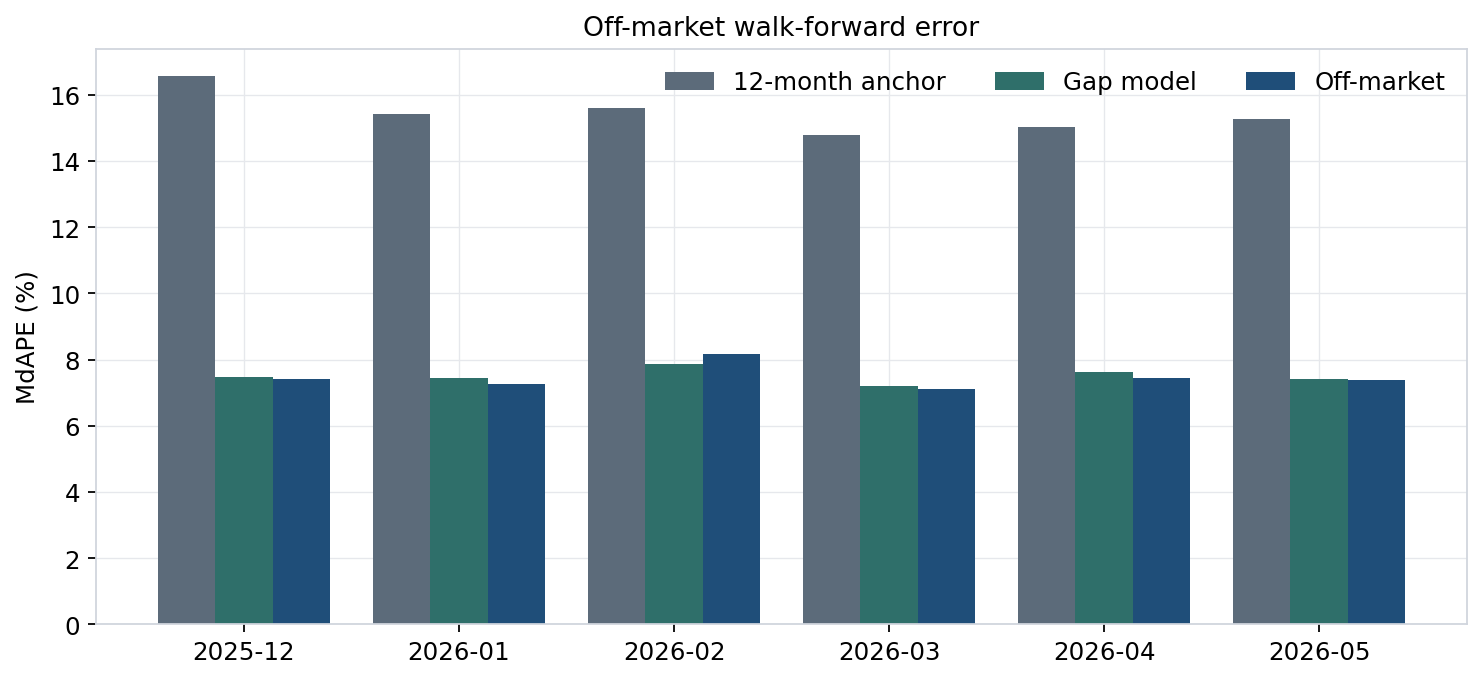
\includegraphics[width=0.92\linewidth]{report_om_mdape.png}
\captionof{figure}{Walk-forward MdAPE by sale month. The 12-month community anchor is the baseline. The gap model prices the home as that anchor times a tree. February is the month the gap model is lower.}
\label{fig:om-walk}
\end{center}

\section{Specifications we measured and did not keep}

Choices were frozen on July--November 2025, or confirmed on the walk-forward. A win on one frozen six-month cut was not enough.

\subsection{List-aware}
\label{app:drop-la}

\begin{center}
\small
\begin{tabular}{p{6.2cm}p{8.8cm}}
\toprule
Candidate & What happened \\
\midrule
Remarks, text components & Developmental MdAPE \(4.85\) against \(4.83\). Left out. \\
A level shift after the tree & Best one-origin cell, \(4.40\). Walk-forward signed error \(-1.75\). Not adopted. \\
Rotated coordinates, clusters, 10 nearest sales & Developmental MdAPE \(4.52\)--\(4.53\). No improvement. \\
\bottomrule
\end{tabular}
\end{center}

\subsection{Off-market}
\label{app:drop-om}

\begin{center}
\small
\begin{tabular}{p{6.2cm}p{8.8cm}}
\toprule
Candidate & What happened \\
\midrule
Price \(=\) community anchor \(\times\) a tree & Walk-forward MdAPE \(7.50\), against \(7.45\). Kept as the challenger. \\
Separate house and condo shifts & \(8.18\) against \(8.17\) for one shift, on the inner screen. \\
Quantile loss at the median & Walk-forward MdAPE \(7.53\), behind squared error. \\
A land term and a drifting city forecast & The inner screen turned both off. \\
All-history community \$/sqft & MdAPE \(16.42\), signed \(+11.97\%\). Stale, and high. \\
\bottomrule
\end{tabular}
\end{center}

\end{document}
